\en

\section{Tool functionalities}
\label{subsec:func}

We propose three main functionalities for the user in the tool, called duplication explorer,
function information, and duplication relatory. Each of the functionalities receives its 
adequated parameters to execute, except an optional parameter shared by all of them, which 
is minimum similarity per query. The minimum similarity per query is not the same as the 
minimum similarity presented in \ref{subsec:setup}, as it enables a volatile change in the minimum 
similarity interest in a query-specific context. There is an explanation of each of the 
main functionalities in this section.

\subsection{Duplication explorer}

The duplication explorer is the principal functionality of our tool. The functionality's
purpose is to expose the user to the duplicated function pairs found by our tool. We 
implement optional filter methods to enable more complex queries, as described below. 
Figure \ref{fig:explorer_ex} demonstrates the functionality usage.

\begin{itemize}
	\begin{item}
		\textbf{Sorting filter:} This filter enables the user to sort the results by the 
		similarity of the function pairs or by the number of duplicated lines. By default, 
		the tool sorts by similarity, and the user can pass a sort parameter to change 
		the sorting method.
	\end{item}

	\begin{item}
		\textbf{Limiter filter:} This filter receives a number parameter named limiter 
		by the user, which limits the number of results shown to the user by this given number.
	\end{item}

	\begin{item}
		\textbf{Pattern filter:} This filter makes the explorer ignore every pair 
		of duplicated functions that do not match a pattern given by the user as a parameter.
		We say that a function matches a pattern if the string formed by the concatenation 
		of the relative path of the code file plus the function name contains the pattern 
		as a substring. The user can define if both functions or at least one of the 
		functions in the pair need to match the pattern by giving a specific parameter.
	\end{item}
\end{itemize}

\begin{figure}
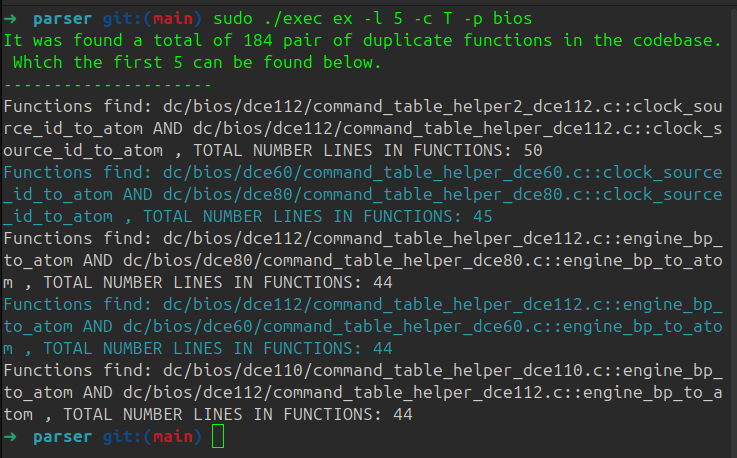
\includegraphics[scale=0.5]{explorer_example}
\caption{Example of the \textit{duplication explorer} functionality of the proposed tool in action.}
\label{fig:explorer_ex}
\end{figure}


\subsection{Function information}

\label{subsec:functioncommand}

The Function information purpose is to give more in-depth information about a specific 
function. The functionality receives a function the user is interested in and then 
informs the user about the relative path, the function name, and the lines the function 
is defined for the function the user is interested in and for every function that is a 
duplication of the given function. There can be multiple functions with the same name 
in a codebase. To distinguish them, we receive a pattern string from the user, and we 
use the first function to find one that matches the given pattern. We say that a 
function matches a pattern if the string formed by the concatenation of the relative 
path of the code file plus the function name contains the pattern as a substring. 
Figure \ref{fig:function_ex} demonstrates the functionality usage.

\begin{figure}
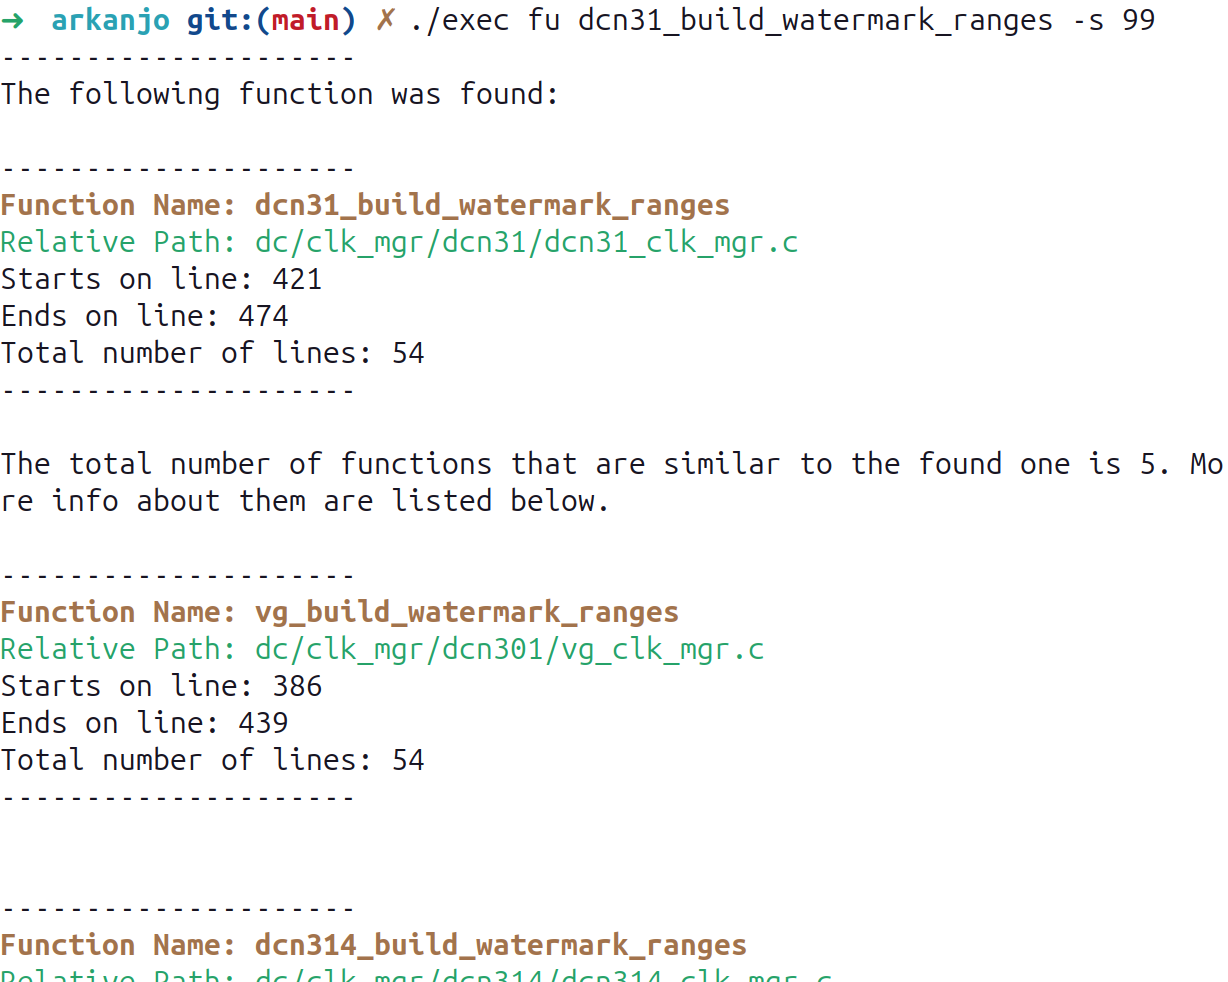
\includegraphics[scale=0.5]{function_example}
\caption{Example of the \textit{function information} functionality of the proposed tool in action.}
\label{fig:function_ex}
\end{figure}


\subsection{Duplication relatory}

The duplication relatory purpose is to give an overview of the input codebase. 
The functionality extracts how many lines of duplicated code per folder in the 
codebase and presents it to the user in a reasonable format. To extract the 
information, we use the Code Duplication Database to list the duplicated functions 
and the temporary code to know how many lines the duplication functions have. 
Figure \ref{fig:relatory_ex} demonstrates the functionality usage. 
(DO I TALK ABOUT THE TRIE USAGE TO MAINTAIN THE HIERARCHICAL TREE STRUCTURE? I THINK NOT)

\begin{figure}
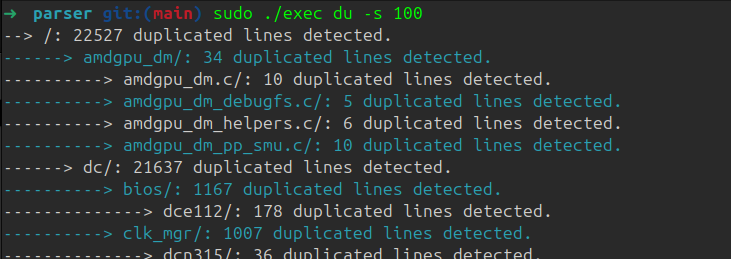
\includegraphics[scale=0.5]{relatory_example}
\caption{Example of the \textit{duplication relatory} functionality X of the proposed tool in action.}
\label{fig:relatory_ex}
\end{figure}





